\section{Toric Variety}
\label{sec:toric-variety}

%% Subsection
\subsection{Toric variety}
\label{subsec:toric-variety}
    A toric variety is a variety that contains algebraic torus $T^n$ as an open dense subset,
    with an action of $T^n$ extended to the variety. 
    The formal definition is as follows:
    \begin{definition}
    \label{def:toric-variety}
	    A \emph{toric variety} $X$ is a complex algebraic variety 
	    containing an algebraic torus $T = (\C^\ast)^r$ as a dense open set,
 	    together with an action of $T$ on $X$ whose restriction to $T \subset X$ is just the multiplication on $T$. 
    \end{definition}

    \begin{example}
	    The complex projective space $\C\P^2$ is defined as $(\C^3 - \{(0,0,0)\})/\C^\ast$.
	    In this space, we can identify the torus $T = \{(1, t_1, t_2) | t_i \in \C^\ast\} \simeq (\C^\ast)^2$ in $\C\P^2$.
	    Note that the action of $T$ on $\C\P^2$ is given by, 
	    \[ (t_1, t_2) \cdot (x_1, x_2, x_3) = (x_1, t_1 x_2, t_2x_3)\]
	    for $(t_1, t_2) \in T, (x_1, x_2, x_3) \in \C\P^2$. 
	    Hence $\C\P^2$ is a toric variety.
    \end{example}


%% Subsection
\subsection{Fan}
\label{subsec:fan}
    Now we define the structure of a fan from cones, or convex rational polyhedral cones:
    \begin{definition}
    \label{def:strong-convex-rational-polyhedral-cone}
	    Let $N$ be a lattice.
	    A strong convex rational polyhedral cone $\subseteq N = N \otimes \R$ 
	    is a set 
	    \[
	    \sigma = \{a_1 v_1 + a_2 v_2 + \ldots + a_k v_k | a_i \ge 0\}
	    \]
	    generated by a finite set of vectors $v_1, \ldots, v_k$ in $N$ such that $\sigma \cap (-\sigma) = \{0\}$.
    \end{definition}

    \begin{figure}
	\centering
	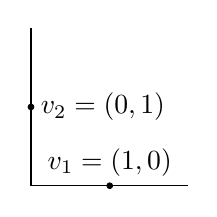
\begin{tikzpicture}
		\draw[black, thin] (0, 0) -- (2, 0);
		\draw[black, thin] (0, 0) -- (0, 2);
		\filldraw[black] (1,0) circle (1pt) node[anchor=south] {$v_1 = (1, 0)$};
		\filldraw[black] (0,1) circle (1pt) node[anchor=west] {$v_2 = (0, 1)$};
	\end{tikzpicture}
    \caption{Four cones for $N$ with rank $2$.}
    \label{fig:example-cones}
    \end{figure}

    In the Figure \ref{fig:example-cones}, the four cones spanned by the sets $\{(0, 1), (1, 0)\}$ are: $\{(0, 0)\}; \{(1, 0)\}; \{(0, 1)\}; \{(1, 0), (0, 1)\}$. 

    Cones constitute fans if certain conditions on the faces hold on these cones and thus give the definition of a fan:
    \begin{definition}
        A collection $\Sigma$ of strongly convex rational polyhedral cones in $N \R$ is called a \emph{fan} if 
	    \begin{enumerate}
		\item[(1)] each face of a cone in $\Sigma$ is also a cone in $\Sigma$, and 
		\item[(2)] the intersection of two cones in $\Sigma$ is a face of each. 
    	\end{enumerate}
    \end{definition}
    This means that all the cones in a fan are closed under intersection and taking faces. 

%% Subsection 
\subsection{Connection between toric varieties and fans}
\label{subsec:toric-variety-fan}
    Toric varieties and fans are tightly connected in the sense
    that we can construct a toric variety from a fan structure and vice versa. 
    Let us find the fan from a simple toric variety $\C\P^2$.
    In order to find a fan -- a collection of cones that live in $N_{\R}$, we start from the lattice itself $N$.
    It is known that there exists a one-to-one correspondence between cones in a fan and $T$-invariant subvarieties 
    as closures of $T$-orbits. 
    Although the details of this proof is not provided here, 
    we exploit this fact and start from finding the $T$-invariant subvarieties.
    Then we try to can find the corresponding cones for each $T$-invariant subvariety.

    Let $T$ be the torus $\{(1, t_1, t_2) | t_i \in \C^\ast\} \simeq (\C^\ast)^2 \subset \C\P^2$.
    Consider the lattice $N = \hom(\C^\ast, T)$ 
    such that elements of $N$ are homomorphisms $\psi: \C^\ast \rightarrow T$,
    which are called one-parameter subgroups, with the only parameter $t$. 
    We claim that the lattice $N = \hom(\C^\ast, T) \cong \Z^2$ 
    by the map $\phi: \Z^2 \mapsto N$ defined as follows:
    \[
    \phi(a, b) \mapsto (t \mapsto (t^a, t^b))
    \] 
    where $(a, b) \in \Z^2, t \in \C^\ast$.

    Let $f$ be the induced inclusion map $f: \C^\ast \rightarrow \C\P^2$ defined as $f(t) = \psi(t) \cdot 1_{\C\P^2}$. 
    Note that image of $f$ is still entirely contained in $T$.
    We want to find sets that are $T$-invariant, or invariant under action by $T$. 
    From group theory, we know that these are called $T$-orbits.
    Taking the closures of $T$-orbit on images of $f$ as $t \rightarrow 0$, 
    we obtain $T$-invariant 
    \[Z_\psi = \overline{T \cdot \lim_{t \rightarrow 0} f(t)}.\]

%% Subsection 
\subsection{Example of constructing a toric variety from a fan}
\label{subsec:contructing-toric-variety}
    Let us see an example by taking a lattice point $(a, b) = (0, 1)$.
    For any $x \in \C^\ast$, $\psi(x)= (x^0, x^1) = (1, x) \in T$. Then $f(x) = (1, 1, x) \in \C\P^2$. 
    Then $\lim_{x \rightarrow 0} f(x) = (1, 1, 0) \in \C\P^2$.
    The orbit of $T$ acting on $\lim_{t \rightarrow 0} f(x)$ is $\{(t_1, t_2) \cdot (1, 1, 0)\} = \{(1, t_1, 0)\} \in \C\P^2$
    where $(t_1, t_2) \in T$.
    Thus, we obtain the line $\{t_2 = 0\}$. 

    We can see from the above example that the relationship amongst $a, b, 0, 1$ are determinant of the cone,
    and these relationships divide the space into different areas,
    each corresponds with a cone. 
    We can then glue all the cones together to find fan. 
